\documentclass{exam}

\usepackage{graphicx}
\usepackage[T1]{fontenc}
\usepackage{wrapfig}
\usepackage{siunitx}

\graphicspath{ {../res/} }

\title{Triathlon - Physics}
\author{Olympiad Maths}
\date{February 15-18, 2022}

\pagestyle{plain}
\marksnotpoints

\begin{document}
\large
\maketitle

\begin{center}
    \vspace{-10pt}
    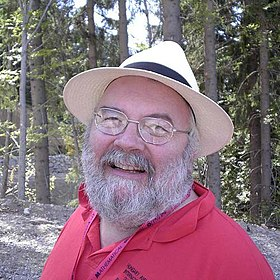
\includegraphics[height=100pt]{geoffsmith}
    \vspace{-10pt}
\end{center}

\section* {Instructions}

Read these before attempting the questions.

\subsection*{Time: 2 hours}

\subsection*{Format}
This paper is split into \textbf{three sections} worth 20, 30 and 30 marks respectively.\\
The first consists of several short questions, the second section requires more thought and the third is on a single theme.\\
Generally the paper is arranged in \textbf{increasing difficulty}.

\subsection*{Philosophy}
The aim of this paper is to test your applied thinking. (And also to be fun!)\\
Do not expect to complete all of the questions; pick ones that you think you will enjoy the most.\\
Some questions have no single correct answer and require you to THINK.

\subsection*{Clarity}
Clarity of working is key - make clear what you assume / approximate.\\
In later questions the answer is irrelevant as long as you have displayed clever thinking and explained your approach.\\
Draw diagrams!!!!!!!!!!!!!

\subsection*{Knowledge required}
Knowledge of GCSE physics is assumed. Useful formulae outside of GCSE are given to you. Section 3 requires A level calculus.

\subsection*{Calculators}
You are allowed a scientific calculator.

\subsection*{Submission}
Submit your paper by dm to
{\fontfamily{cmss}\selectfont e=pi=3\#5257}
before \textbf{23:59 on Friday 18th February}.\\
Please scan in then send as a \textbf{single PDF}. Online tools are available for this.\\
On the front page, write your \textbf{discord ID} (right click username -> copy ID).\\
After submission, you can be added to a channel to discuss the questions. Please don't discuss them outside of that channel.

\centering

\vspace{\stretch{1}}
\section*{Important Constants}
\vspace{20pt}
\begin{tabular}{ c|c|c } 
    \textbf{Constant} & \textbf{Symbol} & \textbf{Value} \\ 
    \hline &&\\
    Elementary charge & $e$ & $1.60\times10^{-19}$ \si{C} \\
    Acceleration of free fall at Earth's surface & $g$ & $9.81$ \si{m.s^{-2}} \\
    Mass of an electron & $m_e$ & $9.11\times10^{-31}$ \si{kg} \\
    Mass of a neutron & $m_n$ & $1.67\times10^{-27}$ \si{kg} \\
    Mass of a proton & $m_p$ & $1.67\times10^{-27}$ \si{kg} \\
    Radius of a nucleon & $r_0$ & $1.2\times10^{-15}$ \si{m} \\
    Planck constant & $h$ & $6.63\times10^{-34}$ \si{Js} \\
    Gravitational constant & $G$ & $6.67\times10^{-11}$ \si{m^3.kg^{-1}.s^{-2}} \\
    Boltzmann constant & $k$ & $1.38\times10^{-23}$ \si{JK^{-1}} \\
    Molar gas constant & $R$ & $8.31$ \si{J.mol^{-1}.K^{-1}} \\
    Avogadro's constant & $N_A$ & $6.022\times10^{23}$ \si{mol^{-1}} \\
    Mass of the Earth & $M_E$ & $5.97\times10^{24}$ \si{kg} \\
    Radius of the Earth & $R_E$ & $6.38\times10^6$ \si{m} \\
    Speed of light in free space & $c$ & $3.00\times 10^8 $ \si{m.s^{-1}} \\
    Speed of sound in air & $c_s$ & $340$ \si{m.s^{-1}} \\
\end{tabular}
\vspace{\stretch{1}}

\newpage\centering
\section*{Useful Formulae}
$$ T_{(K)} = T_{(^\circ C)} + 273 $$
$$ \text{Force due to gravity: } F = \frac{Gm_1m_2}{r^2} $$
$$ \text{Ideal gas: } PV = nRT $$
$$ \text{Volume of sphere: } V = \frac{4}{3} \pi r^3 $$
\vspace{5pt}
Equations of motion for constant acceleration:\\
$v = u+at$ , $s = \frac{u+v}{2}t$\\
\vspace{5pt}
$s = ut + \frac{1}{2}at^2$ , $s = vt - \frac{1}{2}at^2$\\
\vspace{5pt}
$v^2 = u^2 + 2as$\\

\vspace{20pt}
For $x << 1$:
$$ e^x \approx 1 + x $$
$$ (1+x)^n \approx 1 + nx $$
$$ \sin(x) \approx x \approx \tan(x) $$
$$ \cos(x) \approx 1 - \frac{x^2}{2} $$

\vspace{\stretch{1}}
\textbf{The questions begin on the next page.}\\
\vspace{10pt}
Good luck, and most importantly have fun!
\vspace{\stretch{1}}



\newpage
\section*{Section 1 - Short Answer}
This section is worth 20 marks. The questions are computational.
\vspace{20pt}

\begin{questions}
    \question[2]
    A resistor of resistance $R$ is connected in parallel with a resistance $3R$. What is the effective resistance across both resistors?
    \vspace{\stretch{1}}

    \question[2]
    When light enters from air into diamond, it slows down by about 58.6\%. 
    A ray of light enters into an equilateral triangular prism of diamond parallel to the normal on entry. On exit, what is its angle to the exit normal?
    \vspace{\stretch{1}}

    \question[4]
    Hans Langseth (1865-1927) is known for having the longest beard ever, an astounding 17 feet 6 inches. He started growing it at age 19.\\
    \begin{figure}[h]
        \centering
        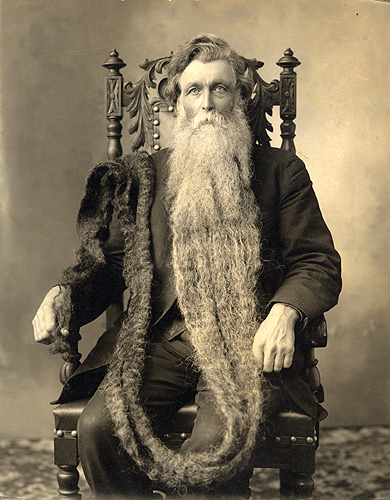
\includegraphics[height=100pt]{hanslangseth}
        \caption{Hans Langseth (From Wikipedia)}
    \end{figure}
    One langseth-beard-second is the distance Hans' beard grows in one second.\\
    One light-foot is the time taken for light to travel one foot.\\
    Convert langseth-beard-seconds per light-foot into meters per second.
    \vspace{\stretch{1}}

    \question[4]
    Drag force is proportional to both $v^2$ and cross sectional area.\\
    Car A has a max speed of 150mph, with a max engine power of 400kW.\\
    Car B has a max engine power of 200kW.\\
    If car B is twice as high as car A and the same width, what is the maximum speed of car B?\\
    \textit{It may help to know that power = force * velocity.}
    \vspace{\stretch{1}}

    \question[4]
    A particle $P$ is at rest on a rough plane inclined at 30$^\circ$ to the horizontal, 5.0m above the ground. It starts to slide down the slope. What is its speed when it reaches the ground?
    Take the frictional force to be $\frac{R}{2}$ , where R is the normal reaction force of the plane on the particle.
    \vspace{\stretch{1}}

    \question[4]
    Sam drops a stone from rest down a well. 2.5 seconds later, he hears a splash. How deep is the well?

\end{questions}



\newpage
\section*{Section 2 - Harder Questions}
This section is worth 30 marks. From now on, the questions will require more thinking.
\vspace{20pt}

\begin{questions}
    \setcounter{question}{6}

    \question[4]
    1.5kg of molten lead is poured into a perfectly insulated container containing 5.0kg of water at $20^\circ$C.
    The final equilibrium temperature is $25^\circ$C.
    What was the initial temperature of the lead?

    \textit{The specific heat capacities of molten lead, solid lead and water, in J/(kg$^\circ$C), are} 140, 127 \textit{and} 4190 \textit{respectively.
    The latent heat of fusion of lead is} 23kJ/kg.
    \textit{Lead melts at} 327$^\circ$C.
    \vspace{\stretch{1}}


    \question[5]
    Suppose you are in space, and looking at the earth. How far away is the best spot to view it from?
    \vspace{\stretch{1}}

    \question
    A ball is thrown from a height $h$ above flat ground at an angle $\theta$ to the horizontal, with speed $|v|$.
    We will derive an expression for the optimum $\theta$ (given $|v|$ and $h$) to maximize the horizontal distance ($d$) travelled by the ball until it hits the ground.

    Let the time the ball is in the air before it hits the ground be $T$.
    \begin{parts}
    \part[1]
    Show that the horizontal distance travelled is $|v|T\cos(\theta)$ .
    \part[3]
    Draw a vector triangle, two sides of which are the intial and final velocities ($v$ and $v_f$ respectively). Show that the third side is $gT$ .
    \part[3]
    Show that the area of this triangle is $\frac{1}{2} gT \times v\cos(\theta)$. Thus show that to maximize $d$, $v$ must be perpendicular to $v_f$ .
    \part[2]
    Hence show that when $d$ is maximized, $\tan(\theta) = \frac{|v|}{|v_f|}$ .
    \part[5]
    Thus find the optimum throwing angle in terms of initial ball speed and height. What is the optimum angle when $h=0$ ?
    \end{parts}
    \vspace{\stretch{1}}

    \question[7]
    A tennis ball of mass $m$ is held on top of a basketball of mass $M >> m$. They are released together at the same time.

    The rebound of the basketball can cause the tennis ball to bounce very high. Show that the tennis ball can bounce up to 9 times its original height.

    \textit{(Reference frames may prove useful.)}
    \vspace{\stretch{1}}

\end{questions}



\newpage
\section*{Section 3 - Themed Questions}
This section is worth 30 marks. We will estimate the temperature at the centre of the Sun.\\
The Sun has mass $M = 2 \times 10^{30}$kg, and radius $R = 7 \times 10^8$m .
\begin{figure}[h]
    \centering
    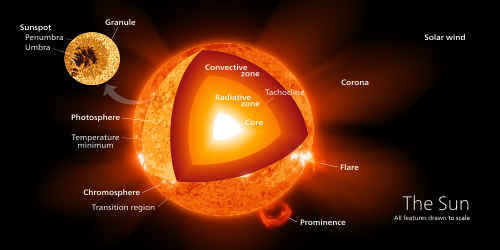
\includegraphics[height=150pt]{sunstructure}
    \caption{Structure of the Sun (From Wikipedia)}
\end{figure}

\raggedright
At a radius $r$ from the centre of the Sun we will consider:
\begin{itemize}
    \item the density, $\rho(r)$
    \item the mass contained within that radius, $m(r)$
    \item the pressure, $P(r)$
\end{itemize}

\vspace{5pt}
\begin{questions}
    \setcounter{question}{10}

    \vspace{\stretch{1}}
    \question[4]
    By considering the pressure difference on a small box of height $dr$ in the Sun, show that
    \begin{equation}
        \frac{dP}{dr} = -\frac{Gm(r)}{r^2} \rho(r)
    \end{equation}
    \textit{(This is known as hydrostatic equilibrium.)}
    \begin{figure}[h]
        \centering
        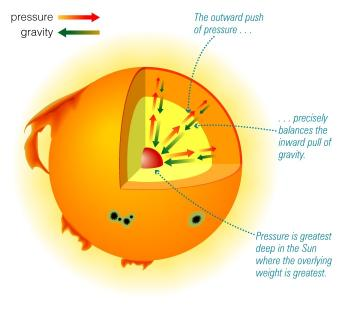
\includegraphics[height=150pt]{hydrostaticeqm}
        \caption{Hydrostatic equilibrium (From National Schools' Observatory)}
    \end{figure}

    \newpage
    \begin{figure}[h]
        \centering
        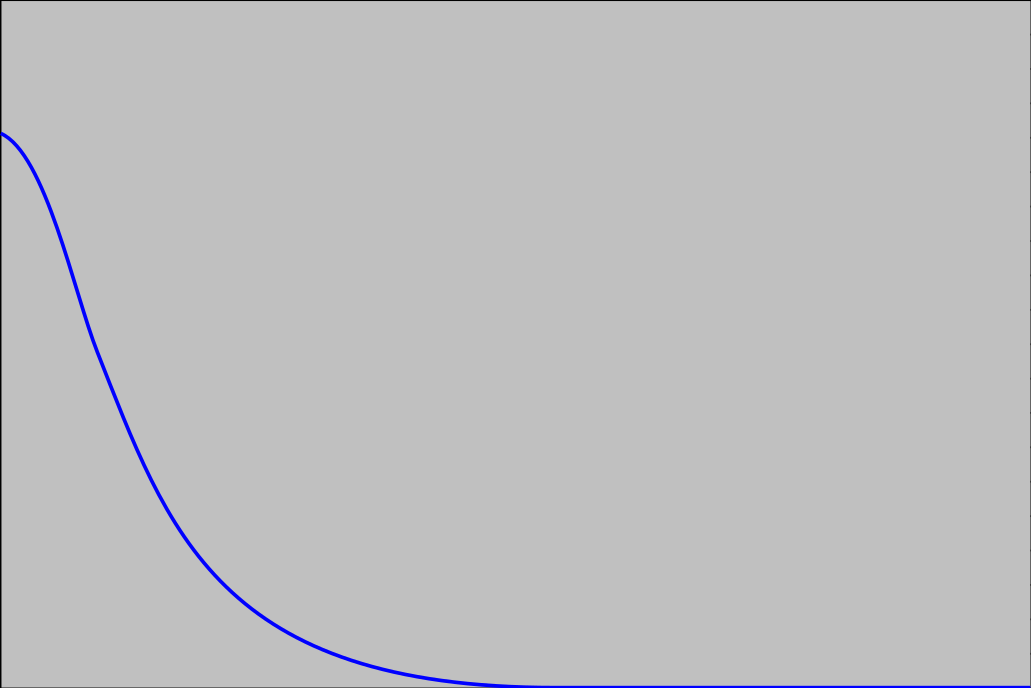
\includegraphics[height=150pt]{sundensityprofile}
        \caption{Density profile of the sun (From Wikipedia)}
    \end{figure}

    Figure 4 shows real data for $\rho(r)$ against $r$, with the $x$-axis being $ 0 \leq r \leq R$ .
    We will model the density profile as the following function:
    $$ \rho(r) = \rho(0)\left(1-\left(\frac{r}{R}\right)^n\right) $$
    For some fixed small $n$ between 0 and 1.
    \question
    \begin{parts}
    \part[1]
    Verify that the model fits Figure 4.
    \part[8]
    Now find $m(r)$ in terms of $r$ (and known constants).
    \part[2]
    Thus write down $\rho(0)$ in terms of known constants.
    \part[10]
    Using equation (1), find $P(0)$ in terms of known constants.
    \part[5]
    Taking $n=0.03$, find the density, pressure and temperature at the centre of the Sun.

    \textit{(Assume the centre of the Sun is made completely of \textbf{ionized} hydrogen gas.)}
    \end{parts}
\end{questions}

\vspace{\stretch{1}}
\centering \LARGE \textbf{END OF PAPER}
\vspace{\stretch{1}}
\end{document}